\documentclass[10pt,a4paper]{article}
\usepackage[utf8]{inputenc}
\usepackage[english]{babel}
%\usepackage{minted}
\usepackage{listings}
\usepackage{xcolor}
\usepackage{graphicx}

%For syntax highlighting
\definecolor{codegreen}{rgb}{0,0.6,0}
\definecolor{codegray}{rgb}{0.5,0.5,0.5}
\definecolor{codepurple}{rgb}{0.58,0,0.82}
\definecolor{backcolour}{rgb}{1,1,1}

%%Sets different parameters
\lstdefinestyle{mystyle}{
	backgroundcolor=\color{backcolour},   
    commentstyle=\color{codegreen},
    keywordstyle=\color{magenta},
    numberstyle=\tiny\color{codegray},
    stringstyle=\color{codepurple},
    basicstyle=\ttfamily\footnotesize,
    breakatwhitespace=false,         
    breaklines=true,                 
    captionpos=b,                    
    keepspaces=true,                 
    numbers=left,                    
    numbersep=5pt,                  
    showspaces=false,                
    showstringspaces=false,
    showtabs=false,                  
    tabsize=4
}
\lstset{style=mystyle}

\title{\bf BCD Addition and Subtraction}
\author{\vspace{-10ex}}
\date{\vspace{-10ex}}
\begin{document}
\maketitle

\begin{minipage}{0.45\textwidth}
        \begin{tabular}{l l}
            \textbf{Expt No:}&7\\
            \textbf{Date :}&09/10/2020
        \end{tabular}
\end{minipage}%
\begin{minipage}{0.45\textwidth}
        \begin{tabular}{l l}
             \textbf{Name:}& Shivanirudh S G  \\
             \textbf{Reg No:} & 185001146 
        \end{tabular}
\end{minipage}
\vspace{1cm}
\hrule

\begin{flushleft}
\subsection*{\textbf{Aim:}} 
To perform BCD addition and subtraction operations in 8086.

\vspace{1cm}
\hrule
\subsection*{\textbf{\underline{BCD Addition}}}

\subsubsection*{\textbf{Algorithm:}}
\begin{itemize}
    \item Move the data segment to the AX register and then move it to the DS register.
    \item Move value of num1 to AL, num2 to BL, carry to CL registers.
    \item Add AL and BL using ADD AL, BL.
    \item Perform Decimal Adjust After Addition using DAA instruction.
    \item Move value of AL to ans.
    \item Jump to label HERE if no carry.
    \item Increment value of CL.
    \item Move value of CL to carry, under label HERE.
\end{itemize}

\newpage
\subsubsection*{\textbf{Program:}}

\begin{table}[htb]
\centering
\resizebox{\columnwidth}{!}{
\begin{tabular}{|l|l|} 
\hline
\textbf{Program}                                                 & \textbf{Comments}                             \\ 
\hline
\hline
assume cs:code, ds:data                                          & Declare code and data segments                \\
\hline
data segment                                                     & Start of data segment                         \\
\hline
num1 db 25H                                                      & Define byte num1 with value 25                \\
\hline
num2 db 36H                                                      & Define byte num2 with value 36                \\
\hline
ans db ?                                                         & Define byte ans for result                    \\
\hline
carry db 00H                                                     & Define byte carry with value 00               \\
\hline
data ends                                                        & End of data segment                           \\
\hline
code segment                                                     & Start of code segment                         \\
\hline
start:~mov ax, data                                              & Move data to AX register                      \\
\hline
mov ds, ax                                                       & Move contents of AX register to DS register   \\
\hline
mov al, num1                                                     & Move value of num1 to AL register             \\
\hline             
mov bl, num2                                                     & Move value of num2 to BL register             \\
\hline
mov cl, carry                                                    & Move value of carry to CL register            \\
\hline 
add al, bl                                                       & AL = AL + BL                                  \\
\hline
daa                                                              & Decimal Adjust after Addition                 \\
\hline
mov ans, al                                                      & Move value of AL register into ans            \\
\hline
jnc here                                                         & Jump to label HERE if no carry                \\
\hline
inc cl                                                           & Increment value of CL                         \\
\hline
here:~mov carry, cl                                              & Move value of CL register into carry          \\
\hline
mov ah, 4ch                                                      & To request interrupt                          \\
\hline
int 21h                                                          & Request interrupt routine                     \\ 
\hline
code ends                                                        & End of code segment                           \\
\hline
end start                                                        &                                               \\
\hline
\end{tabular}
}
\end{table}

\newpage
\subsection*{\textbf{Unassembled code:}}
\begin{figure}[h]
    \centering
    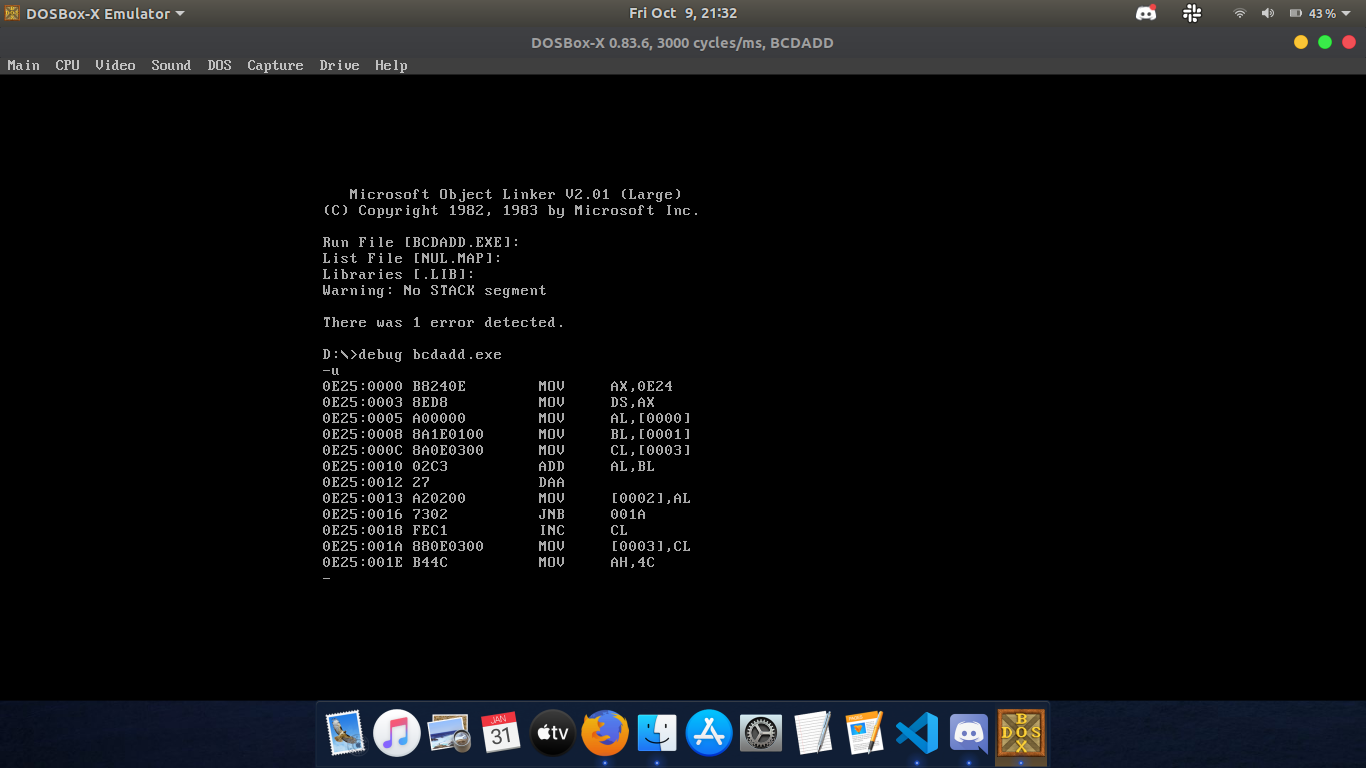
\includegraphics[trim = 100mm 60mm 200mm 120mm, clip, width = \textwidth]{Pics/BAUS.png}
\end{figure}
\subsubsection*{\textbf{Input and Output:}}
\begin{figure}[h]
    \centering
    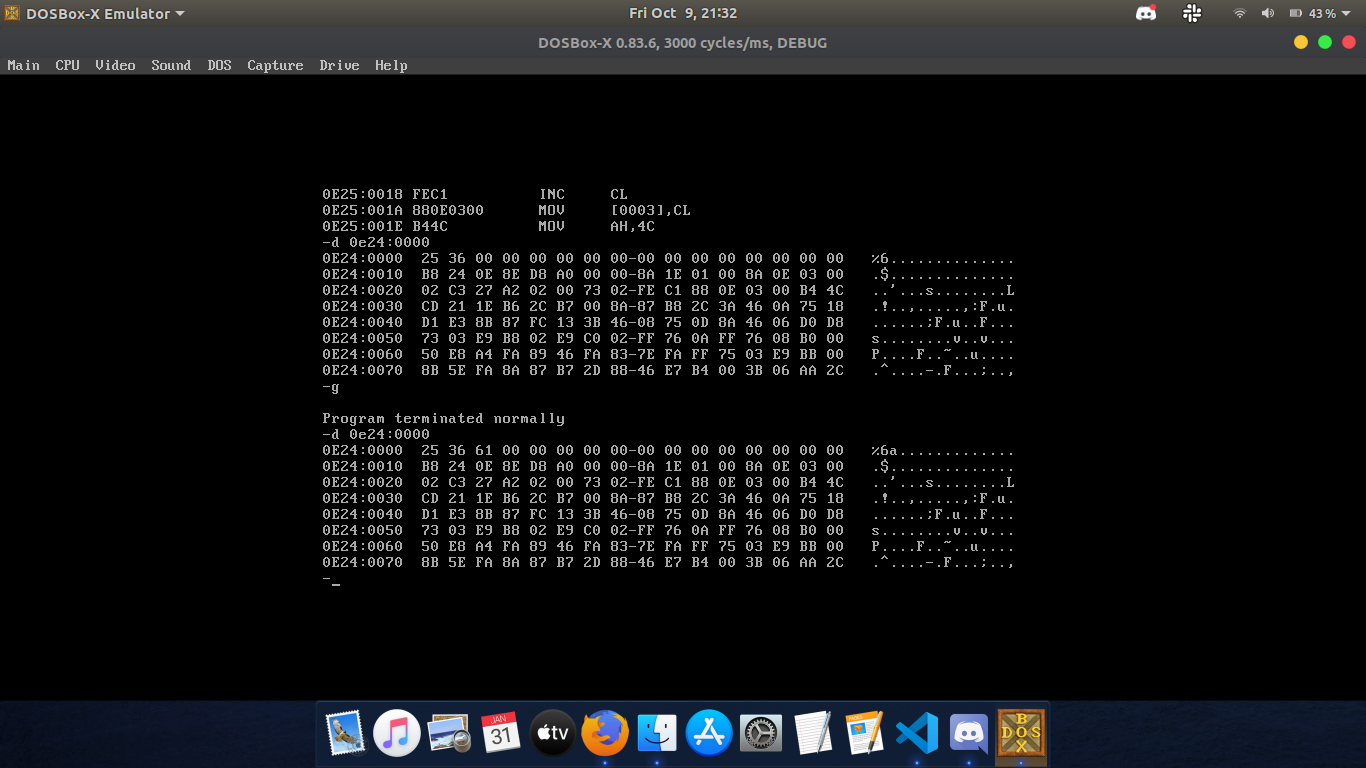
\includegraphics[trim = 100mm 60mm 100mm 80mm, clip, width = \textwidth]{Pics/BAIO.png}
    \caption{ \textbf{Input:} num1: 25, num2: 36; \newline \hspace{1cm}
              \textbf{Output:} ans: 61, carry: 0}
\end{figure}
%-------------------------------------------------------------------------------------------------------------------------------------------
\hrule
\newpage
\subsection*{\textbf{\underline{BCD Subtraction}}}

\subsubsection*{\textbf{Algorithm:}}
\begin{itemize}
    \item Move the data segment to the AX register and then move it to the DS register.
    \item Move value of num1 to AL, num2 to BL, sign to CL registers.
    \item Subtract AL and BL using SUB AL, BL.
    \item Perform Decimal Adjust After Subtraction using DAS instruction.
    \item Jump to label HERE if no carry.
    \item Move value in AL to BL register, 99H to AL register.
    \item Subtract AL and BL using SUB AL, BL.
    \item Add 1 to AL using ADD AL, 01H.
    \item Perform Decimal Adjust after Addition using DAA instruction.
    \item Increment value of CL.
    \item Move value of CL to sign, under label HERE.
    \item Move value of AL to ans.
\end{itemize}

\newpage
\subsubsection*{\textbf{Program:}}

\begin{table}[htb]
\centering
\resizebox{\columnwidth}{!}{
\begin{tabular}{|l|l|} 
\hline
\textbf{Program}                                                 & \textbf{Comments}                             \\ 
\hline
\hline
assume cs:code, ds:data                                          & Declare code and data segments                \\
\hline
data segment                                                     & Start of data segment                         \\
\hline
num1 db 25H                                                      & Define byte num1 with value 25                \\
\hline
num2 db 36H                                                      & Define byte num2 with value 36                \\
\hline
ans db ?                                                         & Define byte ans for result                    \\
\hline
sign db 00H                                                      & Define byte sign with value 00                \\
\hline
data ends                                                        & End of data segment                           \\
\hline
code segment                                                     & Start of code segment                         \\
\hline
start:~mov ax, data                                              & Move data to AX register                      \\
\hline
mov ds, ax                                                       & Move contents of AX register to DS register   \\
\hline
mov al, num1                                                     & Move value of num1 to AL register             \\
\hline             
mov bl, num2                                                     & Move value of num2 to BL register             \\
\hline
mov cl, sign                                                     & Move value of sign to CL register             \\
\hline 
sub al, bl                                                       & AL = AL - BL                                  \\
\hline
das                                                              & Decimal Adjust after Subtraction              \\
\hline                                                           
jnc here                                                         & Jump to label HERE if CF = 0                  \\
\hline
mov bl, al                                                       & Move value of AL to BL register               \\
\hline
mov al, 99H                                                      & Move hex value 99H to AL register             \\
\hline
sub al, bl                                                       & AL = AL - BL                                  \\
\hline
add al, 01H                                                      & AL = AL + 1                                   \\
\hline 
daa                                                              & Decimal Adjust after Addition                 \\
\hline
inc cl                                                           & Increment value of CL                         \\
\hline
here:~mov ans, al                                                & Move value of AL to ans                       \\
\hline
mov sign, cl                                                     & Move value of CL to sign                      \\
\hline
mov ah, 4ch                                                      & To request interrupt                          \\
\hline
int 21h                                                          & Request interrupt routine                     \\ 
\hline
code ends                                                        & End of code segment                           \\
\hline
end start                                                        &                                               \\
\hline
\end{tabular}
}
\end{table}

\newpage
\subsection*{\textbf{Unassembled code:}}
\begin{figure}[h]
    \centering
    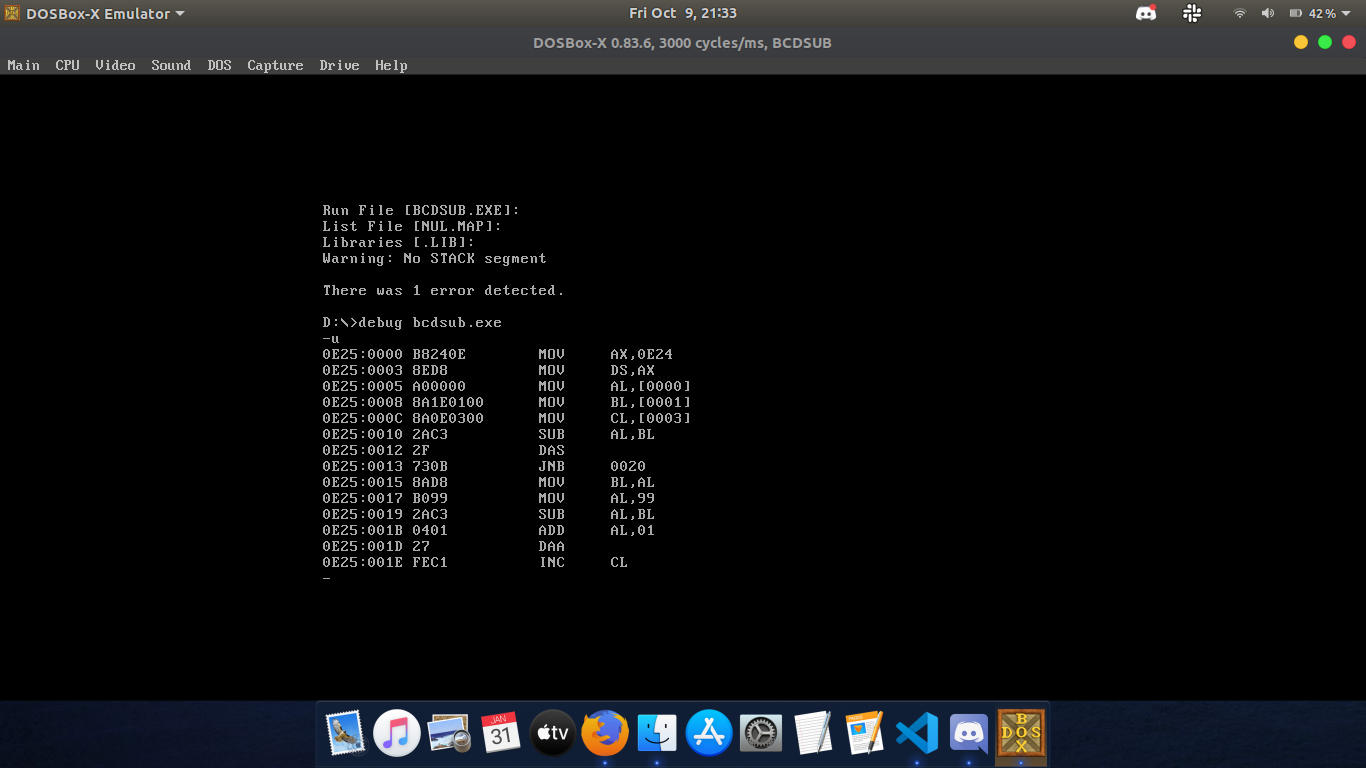
\includegraphics[trim = 100mm 60mm 200mm 120mm, clip, width = \textwidth]{Pics/BSUS.png}
\end{figure}
\subsubsection*{\textbf{Input and Output:}}
\begin{figure}[h]
    \centering
    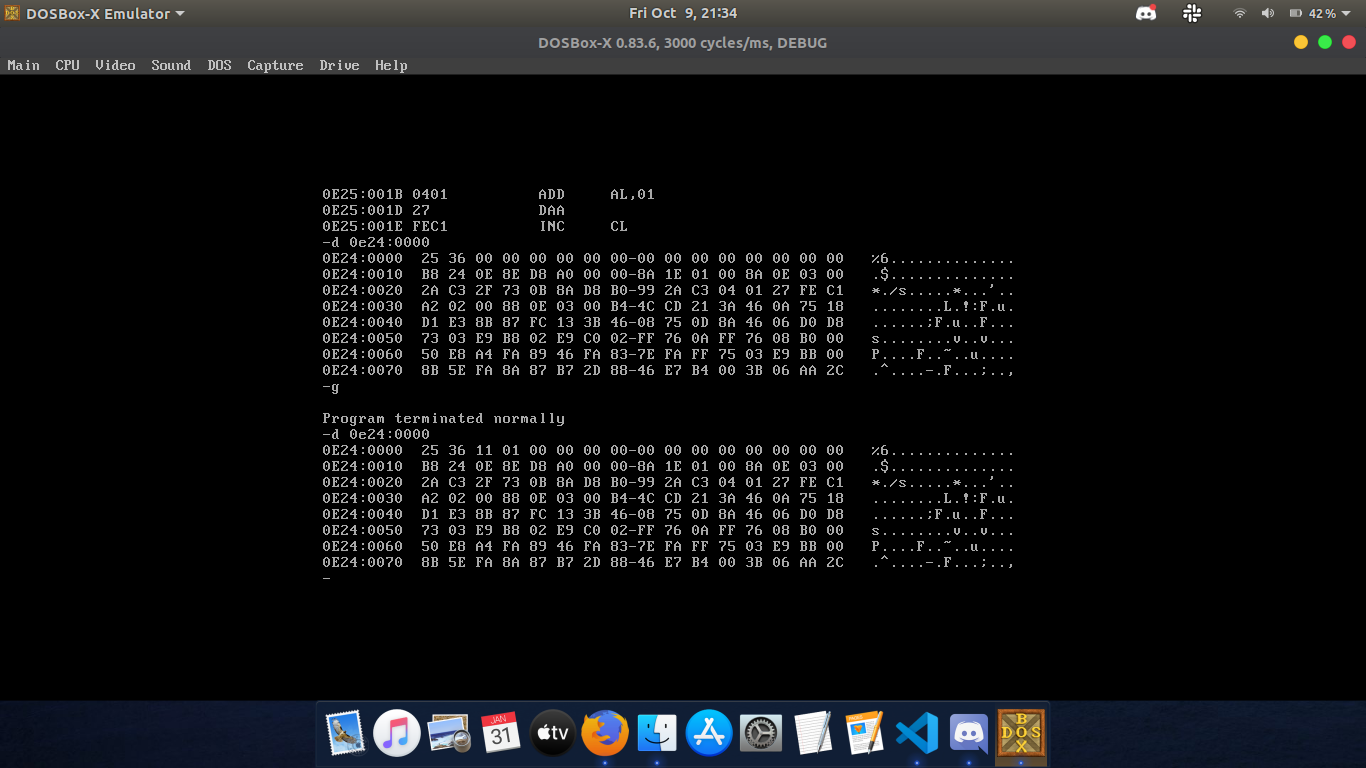
\includegraphics[trim = 100mm 60mm 100mm 80mm, clip, width = \textwidth]{Pics/BSIO.png}
    \caption{ \textbf{Input:} num1: 25, num2: 36; \newline \hspace{1cm}
              \textbf{Output:} ans: 11, sign: 1}
\end{figure}
\hrule
\subsection*{\textbf{Result:}}
The 8086 programs were written to perform BCD addition and subtraction operations, and the results observed.
\end{flushleft}
\end{document}